\documentclass[10pt, a4paper]{article}
\usepackage[latin1]{inputenc}
\usepackage{amsmath}
\usepackage{amsfonts}
\usepackage{amssymb}
\usepackage{graphicx}
\usepackage{xcolor}
\usepackage{hyperref}
\usepackage{booktabs}
\usepackage[normalem]{ulem}


%% Multicolumns
\usepackage{multicol}
\setlength{\columnsep}{1cm}


% Margin to left and middle
\usepackage[margin={2cm,1cm}]{geometry}


\title{Toxic Comment Classification - Report}

\author{Mick van Hulst \and Dennis Verheijen \and Roel van der burg \and Brian Westerweel \and Joost Besseling}

\begin{document}
	\maketitle
	
	
	%% Start multicolumns
	\begin{multicols}{2}
		
		\section{Problem statement}
		We have chosen the toxic comment classification challenge on Kaggle. This challenge consisted of a dataset of around $\sim$160 thousand wikipedia edit comments which had to be classified given six different classes. These classes regard the level of abuse in each comment. Moreover, the classes are not mutually exclusive, which means our problem is a multilabel classification problem.
		
		\section{Dataset}
		
		Both the training and test set provided by Kaggle consist of about 160 thousand comments, a comment id and for the training set, the respective class labels.
		%TODO een voorbeeld sample
		
		One important characteristic of our data is that the set is very imbalanced (figure \ref{fig:imbalance}). This posed many challenges to us.
		
		
		\begin{figure}[h]
			\centering
			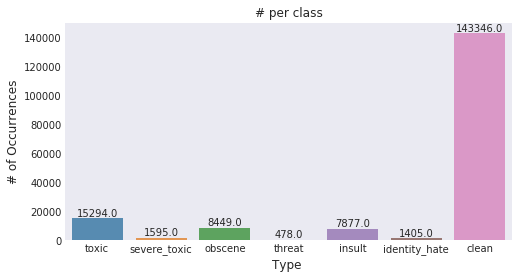
\includegraphics[width=0.5\linewidth]{img/distribution_histogram.png}
		\end{figure}
		
	\end{multicols}
	
	
	\begin{table}[]
		\centering
		\label{my-label}
		\begin{tabular}{|l|l|}
			\hline
			\textbf{Tweet}                                                                                                                                         & \textbf{Class} \\ \hline
			\begin{tabular}[c]{@{}l@{}}Who are you tomorrow? Will you make me smile or just\\ bring me sorrow? \#HottieOfTheWeek Demi Lovato\end{tabular} & 0,0,0,0,0,0   \\ \hline
			\begin{tabular}[c]{@{}l@{}}The maestro ... the legend Roger Federer king of the backhand\\ game one of his best shots\end{tabular}            & 0,0,0,0,0,0  \\ \hline
		\end{tabular}
		\caption{Example Wikipedia edit comments from the Kaggle Toxic Comment classification challenge}
	\end{table}
	
	
	
	%% Start multicolumns
	\begin{multicols}{2}
		
		
		\subsection*{Data Preprocessing}
		The data consists of raw Wikipedia edit comments, so some pre-processing is necessary before using them for training purposes. These preprocessing steps include tokenizing sentences and subsequently converting individual words to lowercase and correct erroneously spelled words. Though  naturally, different algorithms might require different data. While misspelled words might not be good input for some neural networks, the occurrence of misspellings might be a good hand-crafted feature.
		
		\begin{table*}[t]
			\centering
			\begin{tabular}{l|c}
				\toprule
				\textbf{Method} & \textbf{AUC} \\
				\midrule
				Feature Based Approach v1 & 0.60   \\
				Feature Based Approach v2 & 0.53 \\
				Convolutional Neural Network & 0.49 \\
				Vanilla LSTM & 0.52 \\
				Bidirectional LSTM & 0.93 \\
				\bottomrule
			\end{tabular}
			\caption{Summary of the achieved results, the Area Under the Curve (AUC) are computed using Kaggle.}
			\label{table:summary_results}
		\end{table*}
		
		
		\section{Models}
		Several approaches were taken, starting with feature extraction, followed by Neural Network approaches including language modeling with an LSTM and a convolutional network.
		
		\subsection{Feature Extraction}
		Our first approach included mahual feature extraction. The features were handcrafted, such that they are tangible features (i.e. not generated by a Neural Network).
		\subsubsection{Feature Based Approach v1}
		In the first iteration of this approach, more generic features were used:
		\begin{itemize}
			\setlength\itemsep{0px}
			\item Ratio of capitals vs total characters
			\item Ratio of punctuation characters
			\item Total length in characters, words and in sentences
			\item Total amount of some special characters: ?, (, ), ! and some other characters.
			\item Ration and amounts of unique words		
		\end{itemize}
		In total, about ten features were generated. These features were used to train various classifiers, which will be described in section \ref{sec:classifiers}. Each model was evaluated separately. However, as may be noted from the results but in the end, none of these feature based models managed to produce convincing results.
		
		
		\subsubsection{Feature Based Approach v2}
		
		%After a meeting with our supervisor, we thought that a problem with our feature extraction was that we might be using too little features. 
		
		Since we are trying to predict 6 classes separately, and we are using a  complex set, the dimensionality of the set is probably higher than 10. That is why we decided to introduce some extra features.
		
		\begin{itemize}
			\item For a list of swear words (since we are doing \emph{toxic} comment classification), we added a feature denoting whether that particular word occurred in the comment. This list concluded a list of common abuse and spam words, as well as common function words.
			\item  A word-2-vec score per comment is calculated by taking the average word2vec scores of every word in the sentence, normalised by the tf-idf score of each word.
		\end{itemize}
		
		These features increased features from 10 to 80+ but only gave a marginal improvement to the mean-averaged area under the curve (AUC) score.
		
		\subsubsection{Feature-based Classifiers}
		\label{sec:classifiers}
		%	\subsubsection*{MultiLayer Perceptrons}
		\textbf{Multilayer Perceptrons}
		The multilater perceptron (MLP) is a basic neural network, using only fully connected (or dense) layers. In our case, the input consisted of the total number of features, and the output of the 6 classis as last layer, each denoting the probability that that one of the six respective was active for the current sample. 
		
		We experimented with various configurations of this setup. We varied the number of layers, and the width of the hidden layers.
		
		
		%\subsubsection*{Support Vector Machines}
		\textbf{Support Vector Machines}
		We only used a linear kernel, but the learning time of the SVM was so high, that we quickly decided not to investigate this approach further.
		
		%	\subsubsection*{Random Forests}
		\textbf{Random Forests}
		\hl{The random forest classifier also didn't get good results on the small feature set, we have not YET tested it on the big feature set.}
		
		% \subsubsection*{1D Convolutional Network}
		\textbf{1D Convolutional Network}
		Another approach we tried is the 1-dimensional convolutional network. However, because this network showed weak results (merely 0.4902 ROC AUC score) we decided to drop this approach.
		
		\subsection{Neural Networks}
		
		After a small literature study we found a LSTM (Long Short Term Memory) to be the appropriate method in terms of a neural network approach. Because LSTM's are recurrent neural networks, it can learn temporal information, or the context of words in sentences. First we implemented a basic LSTM with a custom reverse dictionary. For this LSTM algorithm we first tried focusing on a top n percentage of common words as we thought that very common words might be influencing the model too much. However, after testing it on the training set, we noticed that the LSTM performed better when using all of the words. And as such, we abandoned this method.
		
		After that, we found a Kaggle kernel for a bidirectional LSTM. This means that we feed the sentence twice to the LSTM, once normally, from front to back, and once flipped. This mode performed better than aforementioned models, so we continued optimizing it.
		
		% TODO plaatje van de Bidirect lstm
		\begin{figure}
			\begin{verbatim}	
			A forward and backwardsentence
			sentence backward and forward A
			\end{verbatim}
			\caption{An example of how the  Bidirectional layer would feed the data to the LSTM}
		\end{figure}
		
		
		
		\section{Conclusion & Reflection}
		Here we briefly discuss some things that stood out during this project.
		
		\textbf{Imbalanced dataset:} The one thing that stood out from our dataset is that it was very imbalanced. This made it hard to test if our model was performing correctly as predicting that every comment was non-toxic already resulted in an accuracy of $\approx 0.96$. This made it hard to train our models as during training time the model quickly returned a small loss.
		
		\textbf{Ensemble Methods} During the first competition, we found out that ensemble models are extremely powerful for machine learning tasks (e.g. during the project presentations some groups used these). We have decided that we also want to use ensemble methods in the next competition. For this competition however, we did not have the correct models to have an efficient ensemble.
		
		\textbf{Collaboration} After this first project we are more accustomed to each of our group members (i.e. knowing each other's strengths/weaknesses). This makes it easier for us to work together and enables us to divide our tasks accordingly. To efficiently work together, we're going to utilize an existing git strategy, such as git flow. Also, we found great benefit in the weekly meetings and thus we're going to continue doing so.
		\begin{thebibliography}{xx}
			\bibitem{abc}
			\textsc{Jagan}, \textit{Stop the S@\#\$ - Toxic Comments EDA},
			https://www.kaggle.com/jagangupta/stop-the-s-toxic-comments-eda
		\end{thebibliography}
		
		
	\end{multicols}
	
\end{document}
